\documentclass[UTF8,a4paper,12pt,autoindent=true,fontset=none,zihao=-4,scheme=chinese,space=auto]{ctexart}
\usepackage{bookmark}%书签
\setCJKmainfont{SimSun}[BoldFont={SimHei}, ItalicFont={KaiTi}, BoldItalicFont={FangSong}]  % 设置SimSun为主中文字体, 加粗, 斜体, 加粗斜体.
\setmainfont{Times New Roman}[BoldFont={Times New Roman Bold}, ItalicFont={Times New Roman Italic}, BoldItalicFont={Times New Roman Bold Italic}]  % 设置Times New Roman为主英文字体, 加粗, 斜体, 加粗斜体.
\usepackage{amsmath}%数学公式
\usepackage{amssymb}%数学符号
\usepackage{mathrsfs}%花体
\usepackage{amsfonts}%字体
\usepackage{amsthm}%定理
\usepackage{enumitem}%列表
\usepackage{bm}%加粗
\usepackage{cite}%引用
\usepackage{hyperref}%超链接
\usepackage{url}%超链接
\usepackage{booktabs}%三线表
\usepackage{caption}%标题
\usepackage{float}%图片位置
\usepackage{xcolor}%颜色
\usepackage{graphicx}%插入图片
\usepackage{listings}%插入代码
% 设置代码块样式
\lstset{
    basicstyle=\ttfamily,
    columns=fullflexible,
    frame=single,
    breaklines=true,
    postbreak=\mbox{\textcolor{red}{$\hookrightarrow$}\space},
    language=SQL,
    keywordstyle=\color{blue},
    commentstyle=\color{gray},    
    rulecolor=\color{black!30},%边框颜色
    stringstyle=\color{red},
    escapeinside={\%*}{*)},
    showstringspaces=false,
    numbers=left,
    numberstyle=\tiny,
    captionpos=b % 设置标题位置, b表示在底部
}
%设置正文样式, 1.5倍行距, 段前段后0.5行, 段落首行缩进2字符
\linespread{1.5}
\setlength{\parskip}{0.5\baselineskip}
\setlength{\parindent}{2em}
%设置三线表样式
\setlength{\heavyrulewidth}{1.5pt}
\setlength{\cmidrulewidth}{0.75pt}
\setlength{\lightrulewidth}{0.5pt}


\begin{document}
\begin{titlepage}
    \centering % 确保居中对齐
    % 居中封面内容
    \vspace{2cm} % 插入垂直间距
    {\Huge \textbf{数据库笔记}} \\
    \vspace{1.5cm}
    {\Large 烂石} \\
    \vspace{2cm}
    % 插入 Logo 图片
    \begin{flushleft}
        \centering % 确保居中对齐
        
\includegraphics[width=0.5\textwidth]{image/logo.jpg} % 左上角 Logo,调整宽度
    \end{flushleft}
    \vfill
    {\large \today}
\end{titlepage}


\section{第一章:绪论}

\subsection{数据库的4个基本概念}
\begin{enumerate}
    \item 数据data
    \item 数据库database,DB
    \item 数据库管理系统DBMS
    \item 数据库系统DBS
\end{enumerate}
\subsection{数据库系统的特点}
\begin{enumerate}
    \item 结构化
    \item 共享性高,低冗余,易扩充
    \item 数据独立性高:物理;逻辑
    \item 由DBMS统一管理和控制
\end{enumerate}
\subsection{数据模型}
\begin{enumerate}
    \item 概念模型-E-R图
    \item 逻辑模型--关系模型
    \item 物理模型
\end{enumerate}
\subsection{数据模型的组成要素:数据结构,数据操作,数据的完整性约束条件}
\begin{enumerate}
    \item 数据结构-静态
    \item 数据操作-动态
    \item 完整性约束条件
\end{enumerate}
\subsection{\texorpdfstring{\color{red}\textbf{重点:数据库系统的三级模式结构:外模式,模式(逻辑模式),内模式}}{重点:数据库系统的三级模式结构:外模式,模式(逻辑模式),内模式}}
\begin{enumerate}
    \item 外模式是用户或应用程序看到的局部数据逻辑结构,也称为用户视图。
    每个外模式为特定用户组定制,屏蔽了数据库的复杂结构。
    例如,不同用户可能通过不同的外模式访问同一数据库的不同部分。
    \item 模式是数据库的全局逻辑结构,定义所有数据实体、属性、关系及约束(如主键、外键)。例如,包含所有表的结构及其联系,是数据库设计的核心蓝图。
    \item 内模式描述数据的物理存储方式,如文件组织、索引结构、数据压缩等。例如,决定数据以B+树索引存储,或使用堆文件方式。
\end{enumerate}
外模式是用户视角,模式是全局逻辑蓝图,内模式是物理存储细节。
\subsection{数据库的二级印象功能与逻辑独立性}
\begin{enumerate}
    \item 外模式/模式:保证了数据的逻独立性
    \item 模式/内模式:保证了~物理独立性
\end{enumerate}

 

\section{第四章:数据库安全性(授权)}
\subsection{不安全因素}
\begin{enumerate}
    \item ,,
    \item ,,,
\end{enumerate}
\subsection{数据库安全性控制}

\subsection{\color{red}\textbf{为什么授权?}}
\textbf{授权是指授予(GRANT)和收回(REVOKE),自主存取控制的方法,为了保护数据库防止不合法使用导致数据泄露更改或破坏}

\subsection{\color{red}\textbf{如何授权:授予GRANT}}
\begin{lstlisting}[language=SQL]
    GRANT 权限 ON 对象类型 对象名 TO 用户名 [WITH GRANT OPTION];
\end{lstlisting}
\begin{description}
    \item[权限] 这些是数据库访问的各种权限。例如 SELECT, INSERT, UPDATE, DELETE, CREATE, ALTER, DROP,以及所有权限的缩写 ALL PRIVILEGES 等等。多个权限之间用逗号分隔。
    \item[对象类型:] 这是数据库中可以授予权限的对象类型。常见的类型包括 TABLE, DATABASE, VIEW, FUNCTION, PROCEDURE 等。
    \item[对象名:] 这是具体的数据库对象的名称。比如,如果是表,则可以写表名。如果是数据库全局权限,则直接使用 *。
    \item[TO 用户名:] 指定接受权限的用户或角色。这里可以使用用户名(可能与数据库的用户系统有关)或角色名。如果需要授予权限给多个用户或角色,可以用逗号分隔。
    \item[WITH GRANT OPTION:] 这是可选的子句,它允许被授予权限的用户也能将这些权限再授予其他用户。如果没有这个选项,则用户只能使用这些权限,而不能再传递给其他人.
\end{description}
\paragraph*{示例}
\begin{enumerate}
    \item 给用户 user1 授予 employees 表的 SELECT 权限:
    \begin{lstlisting}[language=SQL]
        GRANT SELECT ON TABLE employees TO user1;
    \end{lstlisting}
    \item 授予 user1 对整个数据库 testDB 查看所有表(ALL TABLES IN SCHEMA)的SELECT权限:
    \begin{lstlisting}[language=SQL]
        GRANT SELECT ON ALL TABLES IN SCHEMA testDB TO user1;
    \end{lstlisting}
    \item 给用户 admin 授予对数据库的所有权限并允许其传递这些权限:
    \begin{lstlisting}[language=SQL]
        GRANT ALL PRIVILEGES ON DATABASE testDB TO admin WITH GRANT OPTION;
    \end{lstlisting}
\end{enumerate}
\textbf{注意:} SQL不允许循环授权(不能以下犯上)
\subsection{收回授权:收回 REVOKE}
\begin{lstlisting}[language=SQL]
    REVOKE 权限 ON 对象类型 对象名 FROM 用户名 [CASCADE][RESTRICT]
\end{lstlisting}
\paragraph*{权限} 
权限是用户在数据库中的操作许可,例如 SELECT, INSERT, UPDATE, DELETE 等。

\paragraph*{对象类型} 
这里指的是数据库中的对象,如 TABLE, VIEW, SEQUENCE, PROCEDURE 等。

\paragraph*{对象名} 
指定权限语句所作用的特定对象的名称。

\paragraph*{用户名} 
需要从中撤销权限的用户或角色名称。

\paragraph*{CASCADE}
如果指定了 CASCADE,当用户拥有权限再授权给其他用户时,撤销其权限也会撤销所有通过他间接获得的权限。

\paragraph*{RESTRICT} 
(可选的,非必要)如果用户已经将权限再授权给其他用户,将阻止该 REVOKE 操作。
使用 \lstinline|RESTRICT| 是为了确保不会不经意地删除其他用户对这些对象的访问权限。

\paragraph*{示例}
\begin{lstlisting}[language=SQL]
REVOKE SELECT ON TABLE employees FROM bob CASCADE;
\end{lstlisting}
这段语句会撤销用户 `bob` 的 `SELECT` 权限,并且由于使用了 `CASCADE`,任何通过 `bob` 获得的 `SELECT` 权限也会被撤销。

\paragraph*{注意}
\texttt{RESTRICT} 和 \texttt{CASCADE} 只能选择一个,不能同时使用。







\section{数据库完整性}
\subsection{三大完整性}
\begin{enumerate}
    \item 实体完整性:保证每个表中记录的唯一性,通常通过主键约束实现,防止出现空值或重复值。
    \item 参照完整性:确保外键值必须是在主键中存在的值,维护表间数据一致性。
    \item 用户定义完整性:按照特定的业务规则,自定义数据的合法性约束,如自定义检查约束、触发器等。
\end{enumerate}
\section{数据库编程}
\subsection{嵌入式SQL与主语言之间的通信}

嵌入式SQL与主语言(如C、Java等)之间的通信主要通过以下几种方式进行:

\begin{enumerate}
    \item \textbf{SQL $\rightarrow$ 主语言}:
        \begin{itemize}
            \item \textbf{通信区(Communication Area, SQLCA)}:用于报告SQL语句执行的状态和错误信息。SQLCA是一个结构体或类,包含了SQL语句的执行结果、错误码、警告等信息。通过检查SQLCA,主语言程序可以获取SQL语句的执行情况并作出相应的响应。
        \end{itemize}
    
    \item \textbf{主语言 $\rightarrow$ SQL}:
        \begin{itemize}
            \item \textbf{主变量(Host Variables)}:主语言的变量可以直接用在嵌入式SQL语句中,将主语言的数据传递到数据库中。在SQL预处理阶段,这些变量会被相应地绑定到SQL语句中。
        \end{itemize}
    
    \item \textbf{查询结果 $\rightarrow$ 主语言}:
        \begin{itemize}
            \item \textbf{主变量和游标(Host Variables and Cursors)}:查询结果可以通过主变量直接返回,也可以使用游标来遍历返回的结果集。游标允许主语言程序逐行访问SQL查询(如SELECT语句)的结果数据。
        \end{itemize}
\end{enumerate}

\textbf{通信区(SQLCA)}:
\begin{itemize}
    \item SQLCA提供了一套结构化或对象化的方式来访问SQL语句执行后的状态和错误信息。具体的字段可能包括:
        \subitem SQLCODE(SQL代码):指示了执行SQL操作的状态,正值表示警告,负值表示错误。
        \subitem SQLERRM(错误信息):包含了描述错误或状况的文本信息。
\end{itemize}

\textbf{主变量}:
\begin{itemize}
    \item 在嵌入式SQL中,可以声明与外部语言兼容的变量,这些变量可以用作输入参数发送到SQL,也可以作为输出接收查询结果的容器。
\end{itemize}

\textbf{游标(Cursors)}:
\begin{itemize}
    \item 游标是一个控制结构,允许对查询结果集进行逐行或批量操作。它包括声明、打开、获取数据、关闭等几个步骤:
        \subitem \texttt{DECLARE}:声明游标。
        \subitem \texttt{OPEN}:打开游标执行查询。
        \subitem \texttt{FETCH}:从游标中获取一行或多行数据。
        \subitem \texttt{CLOSE}:关闭游标释放资源。
\end{itemize}

\subsection{相关示例代码}
下面是一个用C语言与嵌入式SQL(这里假设是使用了一种支持嵌入式SQL的编译器如Pro*C)的基本示例:

\begin{lstlisting}[language=C]
#include <stdio.h>
#include <string.h>

EXEC SQL INCLUDE SQLCA;

// 主变量声明
int id;
char name[20];

EXEC SQL BEGIN DECLARE SECTION;
int ID;
char NAME[20];
EXEC SQL END DECLARE SECTION;

int main() {
    EXEC SQL WHENEVER SQLERROR GOTO error;

    // 从用户获取ID
    printf("Enter ID: ");
    scanf("%d", &ID);
    
    // 查询语句,使用变量
    EXEC SQL SELECT name INTO :NAME FROM Employee WHERE id = :ID;
    
    // 打印结果
    printf("Employee Name foram ID %d is %s", ID, NAME);
    
    goto end;

error:
    printf("Error: %d - %s", sqlca.sqlcode, sqlca.sqlerrm.sqlerrmc);

end:
    return 0;
}
\end{lstlisting}
\section{数据库设计的步骤}
\begin{enumerate}
    \item 需求分析
    \item 概念结构设计--E-R图
    \item 逻辑结构设计--E-R图->逻辑结构,设计用户子模式
    \item 物理结构设计--设计关系,索引
    \item 数据库实施
    \item 数据库运行和维护
\end{enumerate}
\section{数据库恢复技术}
\subsection{事务的概念}

\section{并发控制}
\subsection{并发控制的基本概念}
并发控制:通过锁机制(悲观控制)或多版本控制(乐观控制)确保事务的一致性和隔离性。\\
封锁:在悲观控制中,事务对数据项加锁,防止其他事务同时访问导致数据不一致。\\
数据不一致性:
\begin{enumerate}
    \item 丢失更新
    \item 脏读
    \item 不可重复读
    \item 幻读
\end{enumerate}
\subsection{封锁的基本概念}
排他锁(X锁/写锁):事务加锁后禁止其他事务对该数据项进行读写。\\
共享锁(S锁/读锁):允许其他事务同时加共享锁读取,但禁止加排他锁进行写操作。\\

\subsection{封锁协议}
\begin{enumerate}
    \item 一级封锁协议:事务对数据项加锁后,直到事务结束才释放锁。
    \item 严格两段锁协议(Strict 2PL):事务在整个执行期间只在结束时统一释放所有锁,避免脏读问题。
    \item 两段锁协议(2PL):事务分为加锁阶段和解锁阶段,加锁阶段期间不释放锁,进入解锁阶段后不能再申请新锁。
\end{enumerate}
\subsection{活锁和死锁}
活锁:多个事务不断响应彼此的请求,导致无法有效推进。\\
死锁:多个事务形成相互等待关系,导致系统僵持。\\
死锁处理方法:
\begin{enumerate}
    \item 死锁检测:构建等待图,检测循环依赖。
    \item 死锁恢复:通过回滚部分事务解除死锁。
    \item 死锁预防:采用资源排序、一次性申请所有资源等策略。
\end{enumerate}
\subsection{可串行化调度}
可串行化调度:事务执行顺序经过调整后效果等同于某一串行顺序,保证数据的一致性。\\

\subsection{两段锁协议(2PL)}
两段锁协议:事务执行分为加锁阶段(不释放任何锁)和解锁阶段(统一释放所有锁)。\\

\subsection{多版本并发控制(MVCC)}
多版本并发控制:通过保存数据的多个版本,使得读操作无需等待写锁,从而提高并发性能。常见于乐观并发控制策略。\\


\section{关系理论}
\subsection{函数依赖}
\noindent 非平凡的函数依赖: 对于函数依赖 $X \rightarrow Y$, 若 $Y \not\subseteq X$, 则称为非平凡的函数依赖.\\
平凡的函数依赖: 对于函数依赖 $X \rightarrow Y$, 若 $Y \subseteq X$, 则称为平凡的函数依赖.\\
完全函数依赖: 若 $X \rightarrow Y$成立, 且对于任意 $X$ 的真子集 $X'$, $X' \rightarrow Y$ 均不成立, 则称 $Y$ 对 $X$ 完全依赖.\\
部分函数依赖: 若 $X \rightarrow Y$成立, 且存在 $X'$ 为 $X$ 的真子集使得 $X' \rightarrow Y$ 成立, 则称 $Y$ 对 $X$ 部分依赖.\\

\subsection{码}
候选码: 一个属性集合,满足该集合的属性闭包等于关系中的所有属性,且任一真子集的闭包不等于所有属性.\\
求候选码的方法:
\begin{enumerate}
    \item 确定必须包含的属性: 只出现在依赖左侧的属性或未在依赖中出现的属性.
    \item 确定可能包含的属性: 同时出现在依赖左右两侧的属性.
    \item 组合构造最小的属性集(候选码),其闭包为整个关系.
\end{enumerate}
例题:
\begin{enumerate}
    \item $R(A, B, C, D, E)$, $F = \{A \rightarrow B, B \rightarrow C, C \rightarrow D, D \rightarrow E\}$, 求候选码.\\
    答案: 候选码为$\{A\}$\\
    证明: $A \rightarrow B \rightarrow C \rightarrow D \rightarrow E$.
    \item $R(A, B, C, D, E)$, $F = \{A \rightarrow B, B \rightarrow C, C \rightarrow D, D \rightarrow E, A \rightarrow D\}$, 求候选码.\\
    答案: 候选码为$\{A\}$\\
    证明: $A \rightarrow B \rightarrow C \rightarrow D \rightarrow E$ 以及 $A \rightarrow D$.
\end{enumerate}
超码: 一个属性集合, 若其闭包包含关系中所有属性, 则称为超码.\\
主码(码): 最小的超码,即去除任一属性后闭包不再等于整个关系的属性集合.\\
主属性: 属于主码的属性.\\
非主属性: 不属于主码的属性.\\
外码: 与其它关系候选码建立关联的属性集合.\\
全码: 关系中所有属性组成的集合.\\
\subsection{范式}
\noindent 第一范式(1NF): 关系中的每个属性都是不可再分的基本数据项.\\
第二范式(2NF): 关系中的每个非主属性完全依赖于任意一个候选码.\\
第三范式(3NF): 关系中的每个非主属性不传递依赖于任意一个候选码.\\
BCNF: 关系中的每个属性都与候选码有直接关系.\\
4NF: 关系中的每个多值依赖都是平凡的或者完全依赖于候选码.\\
判断范式的方法:
\begin{enumerate}
    \item 1NF: 检查是否有多值属性.
    \item 2NF: 检查是否有部分依赖.
    \item 3NF: 检查是否有传递依赖.
    \item BCNF: 检查是否有非平凡的函数依赖.
    \item 4NF: 检查是否有多值依赖.
\end{enumerate}
分解关系的方法:画依赖图分析关系。
从低到高逐步分解,不要跳过步骤。\\
分解关系的目的:
\begin{enumerate}
    \item 保持函数依赖: 保持原关系中的所有函数依赖.
    \item 保持连接性: 保持原关系中的所有元组.
    \item 保持覆盖性: 保持原关系中的所有属性.
\end{enumerate}
\subsection{最小函数依赖集}
求最小函数依赖集的方法:
\begin{enumerate}
    \item 拆分右侧多属性: 若 $X \rightarrow Y$,则 $X \rightarrow Y_i$.
    \item 去除自身求闭包: 若 $X \rightarrow Y$,则 $X$ 的真子集 $X'$ 不能决定 $Y$.
    \item 左侧最小化: 若 $X \rightarrow Y$,则 $X$ 的真子集 $X'$ 不能决定 $Y$.
\end{enumerate}
例题:
设 $R(A, B, C, D, E)$, $F = \{C \rightarrow A, CG \rightarrow BD, CE \rightarrow A, ACD \rightarrow B\}$, 求最小函数依赖集.\\
解析:\begin{enumerate}
    \item 拆分右侧多属性: $CG \rightarrow BD$ 可拆分为 $CG \rightarrow B$ 和 $CG \rightarrow D$.
    \item 去除自身的依赖,求能不能闭包: 保留$C \rightarrow A$,去掉$CG \rightarrow B$,保留$CG \rightarrow D$,去掉$CE \rightarrow A$,保留$ACD \rightarrow B$.
    \item 左侧最小化: $ACD \rightarrow B$ 可最小化为 $CD \rightarrow B$.
    \end{enumerate}
答案: 最小函数依赖集为$\{C \rightarrow A,CG \rightarrow D, CD \rightarrow B\}$.
\subsection{模式分解}
判断无损连接分解的方法:
\begin{enumerate}
    \item 画表格,列出原关系的所有属性.
    \item 画表格,列出分解后的关系的所有属性.
    \item 更新表格,列出所有属性的闭包.
    \item 若闭包相等,则无损连接.
\end{enumerate}
例题:
设 $R(A, B, C, D, E)$, $F = \{A \rightarrow C, C \rightarrow D, DE \rightarrow C, CE \rightarrow A\}$, 求模式分解.\\
解析:
\par 关系模式 \( R(A, B, C, D, E) \) 在函数依赖集 \( F = \{A \rightarrow C, C \rightarrow D, DE \rightarrow C, CE \rightarrow A\} \) 下的 \textbf{3NF 分解} 如下:

\begin{enumerate}
    \item \textbf{DEC(D, E, C)}
    \begin{itemize}
        \item 包含函数依赖 \( DE \rightarrow C \) 和 \( C \rightarrow D \)。
        \item 候选键为 \( DE \),满足 3NF。
    \end{itemize}

    \item \textbf{CEA(C, E, A)}
    \begin{itemize}
        \item 包含函数依赖 \( CE \rightarrow A \) 和 \( A \rightarrow C \)。
        \item 候选键为 \( CE \),满足 3NF。
    \end{itemize}

    \item \textbf{BCE(B, C, E)}
    \begin{itemize}
        \item 包含候选键 \( BCE \),确保无损连接。
        \item 所有属性均为候选键的一部分,满足 3NF。
    \end{itemize}
\end{enumerate}

\textbf{分解步骤说明:}
\begin{enumerate}
    \item \textbf{确定候选键}
    \begin{itemize}
        \item 通过闭包计算,候选键为 \( BCE \)、\( BDE \)、\( BAE \)。所有候选键必须包含 \( B \),因为 \( B \) 无法通过其他属性推导。
    \end{itemize}

    \item \textbf{构造 3NF 关系模式}
    \begin{itemize}
        \item 为每个函数依赖创建关系模式:
        \begin{itemize}
            \item \( A \rightarrow C \) 映射到 \textbf{CEA}(通过合并 \( CE \rightarrow A \))。
            \item \( C \rightarrow D \) 映射到 \textbf{DEC}(与 \( DE \rightarrow C \) 合并)。
            \item 添加候选键关系模式 \textbf{BCE}。
        \end{itemize}
    \end{itemize}

    \item \textbf{验证依赖保持与无损连接}
    \begin{itemize}
        \item 所有函数依赖均被保留在子模式中。
        \item 候选键 \( BCE \) 的存在保证了无损连接。
    \end{itemize}
\end{enumerate}
答案:\\
\textbf{最终分解结果:}
\begin{itemize}
    \item \textbf{DEC(D, E, C)}
    \item \textbf{CEA(C, E, A)}
    \item \textbf{BCE(B, C, E)}
\end{itemize}

该分解满足 3NF,保持所有函数依赖,并确保无损连接。
\section{关系语言}
\subsection{关系代数}
\noindent 集合运算: 
\begin{itemize}
    \item 并: $R \cup S = \{t | t \in R \vee t \in S\}$.
    
    \item 差: $R - S = \{t | t \in R \wedge t \notin S\}$.
    \item 交: $R \cap S = \{t | t \in R \wedge t \in S\}$.
    \item 笛卡尔积: $R \times S = \{t | t = t_1 \cup t_2, t_1 \in R, t_2 \in S\}$.
\end{itemize}
关系运算:
\begin{itemize}
    \item 选择: $\sigma_{\text{条件}}(R)$.
    \item 投影: $\pi_{\text{属性列表}}(R)$.
    \item 连接: $R \bowtie S$.
    \item 除: $R \div S$.
\end{itemize}
\section{SQL语句}
\subsection{SQL语句分类}
\section{事务调度}
\subsection{事务调度的准则}
\begin{enumerate}[label=(\arabic*)]
    \item 一组事务的调度必须保证:
    \begin{enumerate}[label=\alph*.]
        \item 包含的每个事务的操作指令.
        \item 事务的操作指令的执行顺序.
    \end{enumerate}
    \item 并行事务的调度必须保证:
    \begin{enumerate}[label=\alph*.]
        \item 可串行化.
        \item 事务的操作指令的执行结果与它们在某个串行调度中的执行结果相同.
    \end{enumerate}
    \item 判断一个调度是否可串行化的充分条件:
    \begin{enumerate}[label=\alph*.]
        \item 冲突可串行化.
        \item 冲突操作: 两个事务中的操作指令, 一个读, 一个写, 且操作的数据对象相同.
        \item 一个调度是冲突可串行化的, 当且仅当它是冲突可串行调度.
    \end{enumerate}
\end{enumerate}
\subsection{封锁}
\begin{enumerate}[label=(\arabic*)]
    \item X锁: 读写锁, 用于写操作.
    \item S锁: 读锁, 用于读操作.
    \item 封锁协议:
    \begin{enumerate}[label=\alph*.]
        \item 一级封锁协议: 写前加X锁, 读写后解锁,可防止丢失更新.
        \item 二级封锁协议: 写前加X锁, 读前加S锁, 读完释放S锁,事务结束后解锁, 可防止丢失更新和读脏数据.
        \item 三级封锁协议: 读前加S锁, 读写前加X锁, 读写后解锁, 可防止丢失更新, 读脏数据和不可重复读.
        \par 注意:幻读和不可重复读的区别在于, 幻读是由于插入操作引起的, 不可重复读是由于更新操作引起的.
    \end{enumerate}
    \item 两段锁协议: 事务的封锁和解锁操作必须在事务的开始和结束时进行.
\end{enumerate}
\section{数据库设计}
\subsection{ER图}
实体为矩形,属性为椭圆,关系为菱形。联系用线连接实体和关系,表示实体间的联系。关系有一对一、一对多、多对多三种情况。
\begin{figure}[H]
\centering
\includegraphics[width=0.8\textwidth]{image/ER图.jpg}
\caption{ER图}
\end{figure}
\subsubsection{例题}
\begin{figure}[H]
\centering
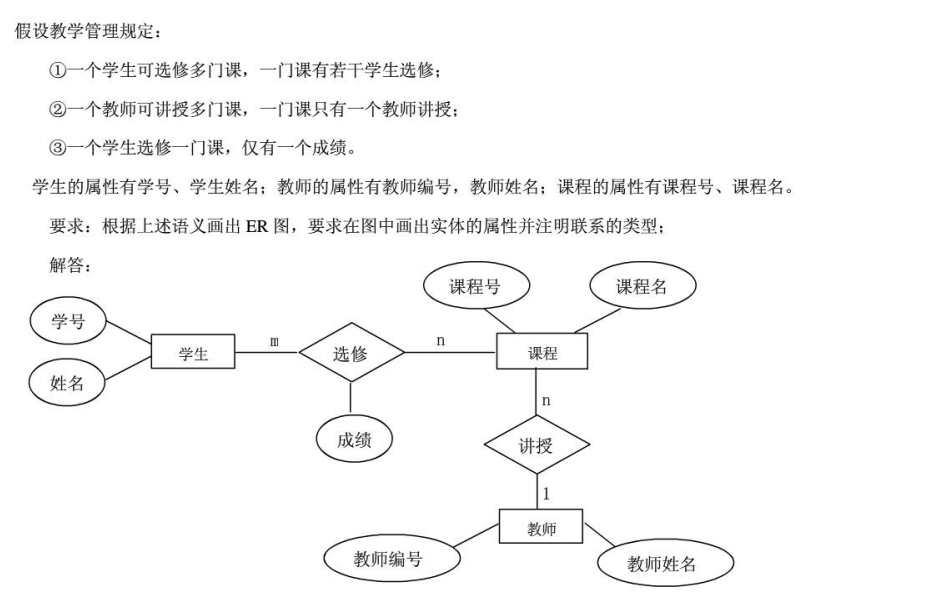
\includegraphics[width=0.8\textwidth]{image/ER图例题.png}
\caption{ER图例题}
\end{figure}


\end{document}

